\chapter{Linear perturbations}\label{ch:linear-perturbations}
\chapterstatus{written}{2026-11-14}

The primordial fluctuations are small, so their evolution until well after recombination follows from Einstein's
equations and the Boltzmann equations of every species expanded to first order around the background of
\cref{ch:background}. The background is translation invariant, so each Fourier mode evolves independently, and
isotropy means that only $k=|\vk|$ matters. This chapter gives the equations solved by the Einstein--Boltzmann solver,
the approximations that make them tractable, and the numerical methods; \cref{ch:cmb-spectra} turns the solution
into observables and \cref{ch:extended-models} describes the perturbations of the models beyond $\Lambda$CDM.

\begin{modulebox}{Cosmology/Perturbations}
Driver: \file{Perturbations.h/.cpp} (class \cls{Perturbations}, namespace \nsp{FML::COSMOLOGY}), \file{Tensors.h/.cpp},
\file{Isocurvature.h}.\par
Model library (namespace \nsp{FML::COSMOLOGY::PERTURBATIONS}, header-only): \file{PerturbationTypes.h},
\file{SpeciesPerturbation.h} and \file{SpeciesPerturbation_<name>.h}, \file{PerturbedFieldEquation.h} and
\file{PerturbedFieldEquation_<name>.h}, \file{QuasiStaticGravity*.h}, \file{PerturbationModel*.h}, \file{Presets.h}.\par
Documentation: \file{Cosmology/Perturbations/README.md}, \file{Cosmology/EinsteinBoltzmannSolver/README.md},
\file{DEVELOPING.md}, the report \file{report/paper.pdf} (Secs.~III, VIII).
\end{modulebox}

\section{Structure of the calculation}\label{sec:pert-structure}

The perturbation module is organised around the observation that photons and baryons, coupled by Thomson scattering,
need special treatment (tight coupling, the line-of-sight sources), while every other species only interacts with
the rest through gravity (or through an explicit coupling to one partner). The solver therefore has
\begin{itemize}
\item a fixed \emph{core}: the baryons $(\delta_b,v_b)$, the photon temperature multipoles $\Theta_0\ldots
      \Theta_{\ell_{\max}}$, the polarization multipoles $\Theta^P_0\ldots\Theta^P_{\ell_{\max}}$ and the potential
      $\Phi$;
\item one \emph{block} per perturbed species of the model (\cls{SpeciesPerturbation}): CDM, massless neutrinos,
      massive neutrinos, scalar fields, dark-energy fluids, and coupled pairs (CDM + dark energy) as one block. A block
      owns its variables, initial conditions, equations, approximation switches and outputs, and communicates with the
      rest only through its \emph{moments} --- $\delta\rho$, $\delta p$, the momentum flux $(\rho+p)\theta/k$ and the
      shear $(\rho+p)\sigma$ --- and the metric $(\Phi,\Psi,\Phi')$ it receives;
\item the \emph{perturbed field equations} of the theory of gravity (\cls{PerturbedFieldEquation}), which compute
      $\Psi$ and $\Phi'$ from the summed moments; scalar--tensor theories add their own variables here.
\end{itemize}
A \cls{PerturbationModel} says which background species get which perturbation block and which field equations to
use; the registry (\file{Presets.h}) builds the model for each name of \cref{tab:bg-models}. A species object is shared
by all modes and threads (no per-mode state). Smooth species ($\Lambda$, $w_0w_a$) get no perturbations.

\section{Metric and Einstein equations}

The scalar perturbations are evolved in the conformal Newtonian gauge with the conventions of
Dodelson \cite{Dodelson2003} and Callin \cite{Callin2006}:
\begin{equation}
\dd s^2=a^2(\eta)\left[-(1+2\Psi)c^2\dd\eta^2+(1+2\Phi)\gamma_{ij}\dd x^i\dd x^j\right],
\end{equation}
where $\gamma_{ij}$ is the spatial metric of curvature $K$. $\Psi$ is the Newtonian potential and $\Phi$ the curvature
perturbation; with this sign convention $\Psi=-\Phi$ without anisotropic stress (the ``Planck'' spatial potential is
$\Phi_P=-\Phi$). We write $\kappa\equiv ck/\Hp$ for the wavenumber in units of the Hubble scale. With all species
contributing through their moments, the $00$ (combined with $0i$) and the traceless $ij$ Einstein equations are
\begin{align}
\Phi'&=\Psi-\frac{c^2k^2}{3\Hp^2}\Phi+\frac{H_0^2a^2}{2\Hp^2}\sum_i\frac{\delta\rho_i}{\rho_{c0}},
\label{eq:pert-einstein1}\\
\Psi&=-\Phi-\frac{12H_0^2a^2}{c^2k^2}\sum_i\frac{(\rho_i+p_i)\sigma_i}{\rho_{c0}},
\label{eq:pert-einstein2}
\end{align}
where the shear moments are normalised so that the photons contribute $(\rho+p)\sigma\to\rho_{c0}\Om_\gamma a^{-4}
\Theta_2$, and in a curved universe $k^2$ is replaced by $k^2-3K$ in the $00$ equation (and in the Poisson equation for the
comoving density). For the standard species in a flat universe \cref{eq:pert-einstein1,eq:pert-einstein2} read
\begin{align}
\Phi'&=\Psi-\frac{\kappa^2}{3}\Phi+\frac{H_0^2}{2\Hp^2}\left[\frac{\Om_{\rm cdm}\delta_{\rm cdm}+\Om_b\delta_b}{a}
+\frac{4(\Om_\gamma\Theta_0+\Om_\nu\mathcal N_0)}{a^2}\right],\\
\Psi&=-\Phi-\frac{12H_0^2}{c^2k^2a^2}\left[\Om_\gamma\Theta_2+\Om_\nu\mathcal N_2\right].
\end{align}
$\Phi$ is evolved and $\Psi$ is algebraic; the Poisson and momentum constraints that are not integrated are used as
tests.

\section{Photons}

The photon distribution is a Planck spectrum with a direction-dependent temperature,
$f=[\exp(p/k_BT(1+\Theta))-1]^{-1}$, and $\Theta(k,\mu,x)$ depends on $\mu=\hat\vk\cdot\hat{\bm p}$. The linearised
Boltzmann equation is
\begin{equation}
\Theta'+i\kappa\mu\Theta=-\Phi'-i\kappa\mu\Psi-\tau'\left[\Theta_0-\Theta+i\mu v_b-\tfrac12P_2(\mu)\Pi\right],
\label{eq:pert-boltzmann}
\end{equation}
with free streaming, the redshift from the changing spatial curvature, the gravitational redshift and Thomson
scattering at the rate $-\tau'$ per unit $x$ (\cref{ch:recombination}), including the Doppler shift off moving
electrons and the angular dependence of the scattering, $\Pi=\Theta_2+\Theta^P_0+\Theta^P_2$. With the Legendre moments
$\Theta_\ell=\frac{1}{(-i)^\ell}\int_{-1}^1\frac{\dd\mu}{2}P_\ell(\mu)\Theta(\mu)$ --- $\delta_\gamma=4\Theta_0$,
$v_\gamma=-3\Theta_1$, and $\Theta_2$ the anisotropic stress --- the hierarchy is
\begin{align}
\Theta_0'&=-\kappa\Theta_1-\Phi',\\
\Theta_1'&=\frac\kappa3\left(\Theta_0-2s_2\Theta_2+\Psi\right)+\tau'\left(\Theta_1+\frac{v_b}{3}\right),\\
\Theta_\ell'&=\frac{\kappa}{2\ell+1}\left[\ell s_\ell\Theta_{\ell-1}-(\ell+1)s_{\ell+1}\Theta_{\ell+1}\right]
+\tau'\left(\Theta_\ell-\frac{\Pi}{10}\delta_{\ell2}\right),\qquad\ell\ge2,
\end{align}
and the polarization hierarchy \cite{Zaldarriaga1995}, which has no gravitational source,
\begin{equation}
\Theta^{P\prime}_\ell=\frac{\kappa}{2\ell+1}\left[\ell s_\ell\Theta^P_{\ell-1}-(\ell+1)s_{\ell+1}\Theta^P_{\ell+1}\right]
+\tau'\left[\Theta^P_\ell-\frac\Pi2\left(\delta_{\ell0}+\frac{\delta_{\ell2}}{5}\right)\right].
\end{equation}
The curvature factors $s_\ell=\sqrt{1-(\ell^2-1)K/k^2}$ are 1 in a flat universe (\cref{sec:pert-curvature}); with
\param{polarization} \code{= false} the polarization is dropped and $\Pi=\Theta_2$.

\paragraph*{Truncation.} The hierarchies are truncated at \param{lmax} (default 8) with the closure of Ma and
Bertschinger \cite{Ma1995}, which assumes the free-streaming solution $\Theta_\ell\propto j_\ell$ for the last
multipole and avoids reflecting power back to low $\ell$:
\begin{equation}
\Theta'_{\ell_{\max}}=\kappa s_{\ell_{\max}}\Theta_{\ell_{\max}-1}-\frac{c(\ell_{\max}+1)\cot_K(\eta)}{\Hp}\Theta_{\ell_{\max}}
+\tau'\Theta_{\ell_{\max}},
\end{equation}
with $\cot_K(\eta)=1/\eta$ when flat. Only the low multipoles enter the line-of-sight sources, so a small $\ell_{\max}$
suffices.

\section{Neutrinos}

\paragraph*{Massless neutrinos} obey the photon hierarchy without collisions, $\tau'=0$, with multipoles
$\mathcal N_\ell$, truncated at \param{lmax_nu} (default 22; 30 changes the spectra by $<5\times10^{-4}$, 12 gives
$0.35\%$ in $P(k)$ at $k=0.3\Mpc^{-1}$). Their quadrupole is a large anisotropic stress in the radiation era, when they
are $41\%$ of the radiation.

\paragraph*{Massive neutrinos.} A massive particle's velocity $cq/\epsilon$ depends on its momentum, so following
Ma and Bertschinger \cite{Ma1995} the distribution is written $f=f_0(q)[1+\Psi_\nu(\vk,\hat n,q,\eta)]$ and expanded
in Legendre multipoles $\Psi_\ell(q)$ at a set of momenta:
\begin{align}
\Psi_0'&=-\kappa\frac q\epsilon\Psi_1+\Phi'\frac{\dd\ln f_0}{\dd\ln q},\\
\Psi_1'&=\frac\kappa3\frac q\epsilon(\Psi_0-2\Psi_2)-\frac\kappa3\frac\epsilon q\Psi\frac{\dd\ln f_0}{\dd\ln q},\\
\Psi_\ell'&=\frac{\kappa}{2\ell+1}\frac q\epsilon\left[\ell\Psi_{\ell-1}-(\ell+1)\Psi_{\ell+1}\right],\qquad\ell\ge2,
\end{align}
with the moments
\begin{equation}
\delta\rho_\nu\propto\int\dd q\,q^2\epsilon f_0\Psi_0,\quad
(\rho+p)_\nu\theta_\nu\propto k\int\dd q\,q^3f_0\Psi_1,\quad
(\rho+p)_\nu\sigma_\nu\propto\frac23\int\dd q\,\frac{q^4}{\epsilon}f_0\Psi_2 .
\end{equation}
For $M\to0$ and $\Psi_\ell=-\mathcal N_\ell\,\dd\ln f_0/\dd\ln q$ this reduces to the massless system. The defaults are
\param{n_q_ncdm} $=8$ Gauss--Laguerre momenta and \param{lmax_ncdm} $=17$ (as CLASS; 16 momenta or $\ell_{\max}=25$
change $C_\ell$ and $P(k)$ by $<3\times10^{-5}$). Deep inside the horizon, $k\eta>$ \param{ncdm_fluid_trigger} $=31$,
the hierarchy is replaced by the fluid approximation of Lesgourgues and Tram \cite{LesgourguesTram2011} for
$\delta_\nu,\theta_\nu,\sigma_\nu$, with the adiabatic sound speed $c_a^2=\frac{w}{3(1+w)}(5-\mathfrak p/p)$ and a
viscosity closure for the shear, as in CLASS. This reduces the system from $\sim190$ to $\sim49$ variables and changes
$P(k)$ by up to $0.3\%$ at $m_\nu=0.3$\,eV, as CLASS's approximation does. Degenerate species are one hierarchy;
different masses (\param{m_nu_list}) each have their own, with outputs \code{delta_ncdm_<i>}, \code{v_ncdm_<i>} and the
totals \code{delta_ncdm}, \code{v_ncdm}.

\section{Cold dark matter and baryons}

CDM is collisionless and non-relativistic, and baryons exchange momentum with the photons:
\begin{align}
\delta_{\rm cdm}'&=\kappa v_{\rm cdm}-3\Phi', & v_{\rm cdm}'&=-v_{\rm cdm}-\kappa\Psi,\\
\delta_b'&=\kappa v_b-3\Phi', & v_b'&=-v_b-\kappa\Psi+\tau'R\,(3\Theta_1+v_b),
\end{align}
with $R=4\rho_\gamma/(3\rho_b)$ ensuring momentum conservation. (In a curved universe the continuity equations carry
the factor $(1-3K/k^2)$ on $\Phi'$ in the conventions of the code.)

\section{Initial conditions}\label{sec:pert-ic}

At \param{pert_x_start} $=-18$ every mode is far outside the horizon in the radiation era. For adiabatic
perturbations, normalised to a primordial comoving curvature perturbation $\mathcal R=1$ (the actual amplitude enters
through $\mathcal P_\mathcal R(k)$ in \cref{ch:cmb-spectra}),
\begin{gather}
\Psi=-\frac{1}{\frac32+\frac25f_\nu},\qquad \Phi=-\left(1+\frac25f_\nu\right)\Psi,\qquad
f_\nu=\frac{\rho_{\rm fs}}{\rho_\gamma+\rho_{\rm fs}},\\
\delta_{\rm cdm}=\delta_b=-\tfrac32\Psi,\quad v_{\rm cdm}=v_b=-\tfrac\kappa2\Psi,\quad
\Theta_0=\mathcal N_0=-\tfrac12\Psi,\quad \Theta_1=\mathcal N_1=\tfrac\kappa6\Psi,\\
\mathcal N_2=-\frac{(cka)^2\Phi}{12H_0^2\Om_\nu}\left(1+\frac{5}{2f_\nu}\right)^{-1},\qquad
\mathcal N_\ell=\frac{\kappa}{2\ell+1}\mathcal N_{\ell-1}\ (\ell\ge3),
\end{gather}
where $\rho_{\rm fs}$ is the density of the free-streaming species (all neutrinos). Each other species gives its
own adiabatic initial conditions. Isocurvature initial conditions are described in \cref{sec:cmb-isocurvature}.

\section{Tight coupling}\label{sec:pert-tc}

At early times $|\tau'|\gg1$ and the scattering terms make the system extremely stiff. The scattering locks
$\Theta_1\simeq-v_b/3$ and suppresses $\Theta_{\ell\ge2}$ by powers of $\kappa/\tau'$. In this regime only
$\delta_{\rm cdm}$, $v_{\rm cdm}$, $\delta_b$, $v_b$, $\Phi$, $\Theta_0$, $\Theta_1$ (and the other species) are evolved, and
\begin{gather}
\Theta_2=-\frac{8}{15}\frac{\kappa}{\tau'}\Theta_1\ \left(\tfrac{20}{45}\text{ without polarization}\right),\qquad
\Theta^P_0=\tfrac54\Theta_2,\qquad \Theta^P_2=\tfrac14\Theta_2,\\
\Theta_\ell=-\frac{\ell}{2\ell+1}\frac\kappa{\tau'}\Theta_{\ell-1}\quad(\ell\ge3).
\end{gather}
The baryon velocity and $\Theta_1$ follow from the second-order expansion of Callin \cite{Callin2006}, which
eliminates the large $\tau'$ terms in favour of the slip $q\equiv3\Theta_1'+v_b'$:
\begin{align}
q&=\frac{-[(1-R)\tau'+(1+R)\tau''](3\Theta_1+v_b)-\kappa\Psi+\left(1-\frac{\Hp'}{\Hp}\right)\kappa(-\Theta_0+2\Theta_2)
-\kappa\Theta_0'}{(1+R)\tau'+\frac{\Hp'}{\Hp}-1},\\
v_b'&=\frac{1}{1+R}\left[-v_b-\kappa\Psi+R\left(q+\kappa(-\Theta_0+2\Theta_2)-\kappa\Psi\right)\right],\qquad
\Theta_1'=\tfrac13(q-v_b').
\end{align}
Tight coupling ends at the first of $|\tau'|<$ \param{tc_tau_min} $=10$, $\kappa/|\tau'|>$ \param{tc_k_over_tau}
$=0.01$ (CLASS's $\tau_c/\tau_k$ trigger; $0.1$ left TT and EE $0.2$--$0.4\%$ low at $\ell=1000$--$2500$) and
$z=$ \param{tc_z_max} $=1700$; the full hierarchy is then initialised from the expressions above.

\paragraph*{Acoustic oscillations and diffusion damping.} At leading order in $1/\tau'$ the photon--baryon fluid is a
driven oscillator,
\begin{equation}
\frac{\dd}{\dd\eta}\left[(1+R_b)\dot\Theta_0\right]+\frac{c^2k^2}{3}\Theta_0=-\frac{c^2k^2}{3}(1+R_b)\Psi
-\frac{\dd}{\dd\eta}\left[(1+R_b)\dot\Phi\right],
\end{equation}
($R_b=1/R$, dots are $\dd/\dd\eta$) with the WKB solution $\Theta_0+(1+R_b)\Psi\simeq A\cos(kr_s)$. At next order
photon diffusion damps the oscillation as $e^{-k^2/k_D^2}$ \cite{HuSugiyama1995},
\begin{equation}
k_D^{-2}=\int_0^\eta\frac{c\,\dd\eta'}{6(1+R_b)n_e\sigma_Ta}\left[\frac{R_b^2}{1+R_b}+\frac{16}{15}\right].
\end{equation}
These analytic results, together with the superhorizon solution of Kodama and Sasaki \cite{Kodama1984}, the
radiation-era potential $\Phi=3\Phi_0(\sin y-y\cos y)/y^3$ ($y=k\eta/\sqrt3$), $\Phi=3/5$ in matter domination for
$\mathcal R=1$, and the growth rate $f\simeq\Om_m(x)^{0.55}$, are the tests of the module (\cref{fig:pert-tests}).

\section{Spatial curvature}\label{sec:pert-curvature}

In a curved universe the plane waves are replaced by eigenfunctions of the Laplacian, $\nabla^2G=-k^2G$, labelled by
$q^2=k^2+K$ and $\nu=q/\sqrt{|K|}$ \cite{HuSeljak1998,LesgourguesTram2014}. Open universes allow every $q>0$; closed
universes are finite and allow only integer $\nu\ge3$ for scalar modes. Three changes follow: $k^2\to k^2-3K$ in the
$00$ Einstein equation, the factors $s_\ell$ in all free-streaming couplings (for a closed universe $s_\nu=0$, so the
hierarchy of mode $\nu$ ends at $\ell=\nu-1$; the physical shear is $\Theta_2/s_2$), and $\cot_K(\eta)$ in the
truncation. The $k$-grid of the code is a grid in $q$; in a closed universe only integer $\nu$ are used, and in an open
universe the grid extends to $q=0.01\sqrt{|K|}$.

\section{Source functions}\label{sec:pert-sources}

After the evolution the temperature and $E$-mode source functions of the line-of-sight integration
(\cref{ch:cmb-spectra}) are built:
\begin{align}
S_T(k,x)&=\gt\left[\Theta_0+\Psi+\frac\Pi4\right]+e^{-\tau}(\Psi'-\Phi')-\frac{1}{ck}\frac{\dd}{\dd x}(\Hp\gt v_b)
+\frac{3}{4c^2k^2}\frac{\dd}{\dd x}\left[\Hp\frac{\dd}{\dd x}(\Hp\gt\Pi)\right],\label{eq:pert-ST}\\
S_E(k,x)&=\frac{3\gt\,\Pi}{4\,[k(\eta_0-\eta)]^2}.\label{eq:pert-SE}
\end{align}
The four terms of $S_T$ are the Sachs--Wolfe term (intrinsic temperature plus the redshift out of the potential at
last scattering), the integrated Sachs--Wolfe term, the Doppler term and the polarization/quadrupole correction. With
\param{store_source_components} they are stored separately (and \param{source_term} selects one for the
$C_\ell$). The derivatives come from integration by parts, which is valid only in a flat universe; in curved
universes the three parts $S_{T0}=\gt(\Theta_0+\Psi)+e^{-\tau}(\Psi'-\Phi')$, $S_{T1}=-\gt v_b$ and $S_{T2}=\gt\Pi/2$
are stored and projected with the radial functions and their derivatives (\cref{ch:cmb-spectra}). The numerator
$3\gt\Pi/4$ of $S_E$ is splined and the factor $1/[k(\eta_0-\eta)]^2$, which diverges today, applied on evaluation.

\begin{implementation}[Implementation: the perturbation solve]
\begin{itemize}
\item \emph{$k$-grid}: \param{pert_n_k} $=400$ modes logarithmically spaced in $[\code{pert_k_min},\code{pert_k_max}]=
      [5\times10^{-5},0.3]\Mpc^{-1}$; with \param{pert_dk_max} $>0$ a log-linear grid (the sources oscillate in $k$ with
      period $\sim2\pi/r_s$, so above $k\approx0.03\Mpc^{-1}$ a linear spacing of $0.004\Mpc^{-1}$ suffices: 112
      modes, the main saving of \code{precision = fast}).
\item \emph{$x$-grid of stored results}: \param{pert_n_x_early} $=300$ points in $[x_{\rm start},-8]$,
      \param{pert_n_x_recomb} $=1200$ in $[-8,-6]$ and \param{pert_n_x_late} $=600$ in $[-6,0]$.
\item \emph{Segments}: the integration is split into segments with fixed equations (tight coupling or not; each
      species' approximation scheme, e.g.\ the neutrino hierarchy or fluid; scalar-field switch points), each solved
      with its own method: \param{method_tc} (RK8PD) during tight coupling, \param{method_full} (GSL's implicit
      \code{msbdf} with a finite-difference Jacobian; $\sim30\times$ faster than RK at $k=0.3\Mpc^{-1}$) after it, and
      \param{method_ncdm} (explicit RK8PD) while the massive-neutrino hierarchy is active, where the dense linear algebra
      of BDF on $\sim190$ variables is $20\times$ slower. Tolerances \param{ode_relerr} $=10^{-8}$,
      \param{ode_abserr} $=10^{-10}$.
\item \emph{Parallelism}: the modes are solved in parallel with OpenMP.
\item \emph{Storage}: all outputs ($\delta_b$, $v_b$, $\Phi$, $\Psi$, $\Phi'$, $\Theta_\ell$, $\Theta^P_\ell$, $\Pi$,
      the species outputs by name, e.g.\ \code{get("delta_cdm", x, k)}, and the sources) are 2D bicubic splines in
      $(x,k)$.
\item \emph{Cost}: $\approx40$\,s for the fiducial model on two cores; massive neutrinos add $\approx7$\,s, curvature
      15--28\,s (mostly in the line of sight).
\end{itemize}
\end{implementation}

\begin{figure}[htbp]
\centering
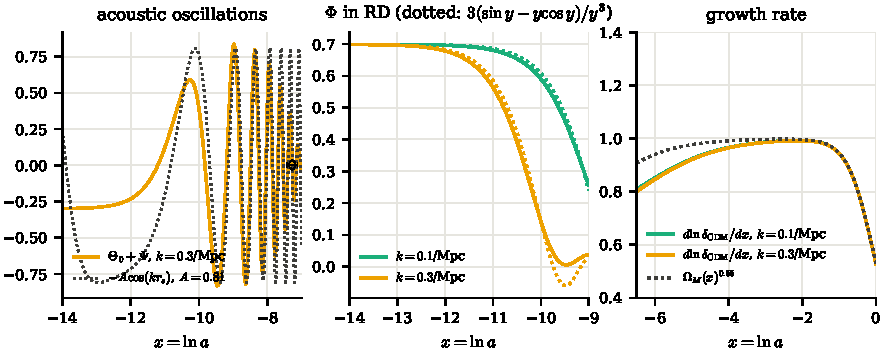
\includegraphics[width=\textwidth]{m3_tests}
\caption{Tests of the perturbations. \emph{Left:} $\Theta_0+\Psi$ for $k=0.3\Mpc^{-1}$ during the radiation era
against $-A\cos(kr_s)$ with the sound horizon of \cref{ch:recombination}. \emph{Middle:} $\Phi$ for modes entering in
radiation domination against the analytic radiation-era solution (dotted). \emph{Right:} the growth rate of
$\delta_{\rm cdm}$ against $\Om_m(x)^{0.55}$. From the solver report.}
\label{fig:pert-tests}
\end{figure}

\begin{figure}[htbp]
\centering
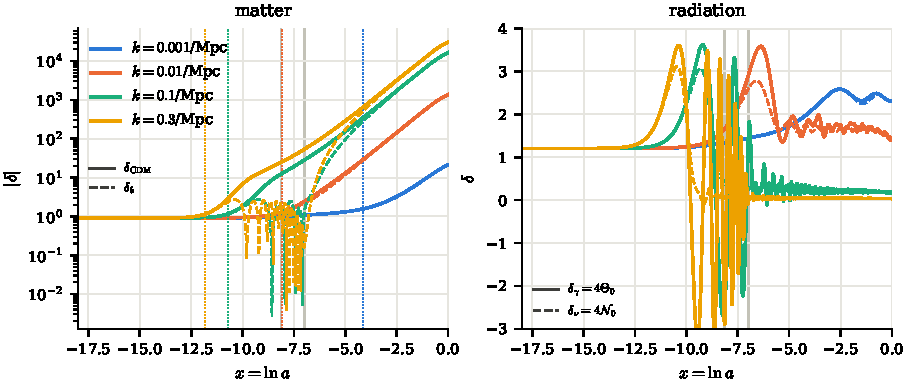
\includegraphics[width=\textwidth]{m3_delta}
\caption{Density perturbations for $k=0.001$, $0.01$, $0.1$ and $0.3\Mpc^{-1}$. \emph{Left:} $|\delta_{\rm cdm}|$
(solid) and $|\delta_b|$ (dashed). \emph{Right:} $\delta_\gamma=4\Theta_0$ (solid) and $\delta_\nu=4\mathcal N_0$
(dashed). Coloured dotted lines mark horizon entry, grey lines equality and decoupling. From the solver report.}
\label{fig:pert-delta}
\end{figure}

\begin{validation}
\begin{itemize}
\item Superhorizon evolution through equality against the Kodama--Sasaki solution; $\Phi\to3/5$ in matter
      domination; the radiation-era potential; the acoustic phase $\cos(kr_s)$; the growth rate $\Om_m^{0.55}$
      (\cref{fig:pert-tests}).
\item The Poisson and momentum constraints, continuity at the tight-coupling switch, free streaming of the neutrino
      multipoles; a nearly massless neutrino ($10^{-4}$\,eV) reproduces the massless one to $4\times10^{-7}$ in $\Phi$.
\item The model library equation by equation against the solver's former species classes ($10^{-8}$; $2\times10^{-7}$
      for the massive neutrinos), at $k=10^{-4},0.05,5\Mpc^{-1}$ and $x=-17,-8,-2,0$.
\item All perturbations against CLASS to $\sim0.1\%$; the end-to-end comparisons are in \cref{ch:cmb-spectra}.
\end{itemize}
\end{validation}

\begin{cppcode}[A custom model and the perturbations of a single mode]
#include <FML/Cosmology/Perturbations/Presets.h>
using namespace FML::COSMOLOGY::PERTURBATIONS;

FML::COSMOLOGY::BACKGROUND::BackgroundParameters p;
p.m_nu_eV = {0.06};
auto model   = make_perturbation_model("horndeski", p, {{"hd_cK", 1.0}, {"hd_cB", 0.6}, {"hd_cM", 0.3}});
auto ctx     = model->context();                       // settings: lmax_nu, lmax_ncdm, n_q_ncdm, ...
auto species = model->species_perturbations(ctx);      // CDM, massless and massive neutrinos
auto gravity = model->field_equation_perturbations(ctx);

// In the full solver (EinsteinBoltzmannSolver.h):
auto ebs = FML::COSMOLOGY::EinsteinBoltzmannSolver::from_file("params/planck2018.ini");
ebs.solve(FML::COSMOLOGY::EinsteinBoltzmannSolver::Stage::Perturbations);
double Phi = ebs.perturbations().get_Phi(-2.0, 0.1 / FML::UTILS::SI::Mpc);   // k in 1/m
\end{cppcode}
